\section{Research Plan and Methodology} \label{sec:rep}

TBD

\subsection{Modeling Concurrency Attacks} \label{sec:model}

% P1: as mentioned in background, a key reason is thread interleavings, 
% so we need to reason about the general patterns we have. Or we say our 
% methodology is just like pattern matching.
P1: TBD.

% P2: pattern 1.
P2: TBD.

% P3: pattern 2.
P3: TBD.

% P4: pattern 3.
P4: TBD.

% P5: how to handle unknow patterns? Just say patterns in our work may spur new 
% patterns. We will continue to find new patterns as well.
P5: TBD.

% \subsubsection{Concurrency Attacks with Three Common Patterns}
% \label{sec:model-pattern}

Goal 1: modeling.

\subsection{Detecting Concurrency Attacks in Testing Phase}\label{sec:detect}

TBD.

\begin{figure}[t]
\centering
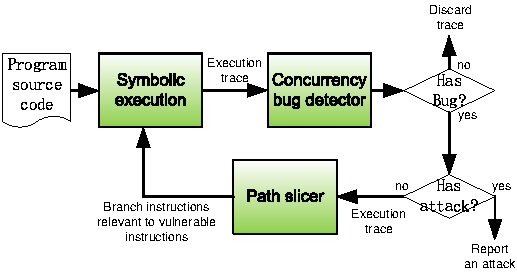
\includegraphics[width=0.5\columnwidth]{figures/detection}
\vspace{-.05in}
\caption{{Workflow of the concurrency attack detection scheme.}} 
\label{fig:detection}
\vspace{-.05in}
\end{figure}

\subsubsection{Workflow of \xxx's Detection Scheme}\label{sec:detect-arch}

% P1: why need a detection scheme. First, capture as many as exploits in 
% testing phase. And call for re-install if there is any potential exploit. Even for 
% old concurrency bugs, it is still necessary because exploits may have already 
% occured and attackers may have already broken in.

% P2: two research questions. Given a concurrency bug, will it lead to an 
% exploit?

% P3: if this bug may lead to an exploit, what inputs may lead to such exploits?

% P4: how to incorporate the patterns in previous section?

% P5: go over the workflow, which is a straight line of boxes. May add some 
% back edges to make it an iterative approach?
 
% \subsubsection{Implementing \xxx's Detection Scheme}\label{sec:detect-impl}
% TBD

\subsubsection{Priliminary work}\label{sec:detect-result}

% P1: we have implemented part of the dangerous operation. pointer NULL 
% derefence. Report the results. FP:FN.

\subsection{Defensing Concurrency Attacks in Deployment Phase} 
\label{sec:defense}

TBD

\subsubsection{Architecture of \xxx's Runtime DefenseInfrastructure} 
\label{sec:defense-arch}

% P1: motivation, why runtime detection is important. We want to mostly avoid 
% exploits by preventing attackers from manipulating the schedules.

% P2: reason 2: when races occur even if Parrot is enforced, we want to have fault-tolerance.

% P3: reason 3: we want survive. checkpoint and re-execute, and diversify the 
% schedules before re-execute. Sell it like a self-healing runtime system.

\subsubsection{Priliminary work} \label{sec:defense-result}

% P1: we have built a replication system. Perf and checkpoint results.

\subsection{Research Plan} \label{sec:rep}
time line. R1 R2.


